\documentclass[12pt]{article}
\usepackage{bm}
\usepackage{graphicx}
\usepackage{gensymb}
\usepackage{float}
\usepackage{siunitx}
\usepackage[a4paper, total={6in, 8in}]{geometry}

\graphicspath{{./../images/}}

\begin{titlepage}

\title{\textbf{Optimum Loft Angle for Greatest Carry Distance}}
\author{\textbf{Group D}\\
		Alison McIntosh\\
		Emily Dark\\
		Henry Archer\\
		Kyle Stewart\\
		Stuart Ballantyne}
\date{}

\end{titlepage}

\begin{document}

\begin{titlepage}
\maketitle
\thispagestyle{empty}
\pagebreak
\end{titlepage}

\pagenumbering{arabic}

\section{Response}
The loft angle of the golf club which maximises the range of the golf ball trajectory is referred to as the optimum loft angle. This investigation consisted of two main parts: the impact of the club, and the flight of the golf ball. The golf ball considered is the Titleist Pro V1, with characteristics outlined under (2.1) Assumptions.

\subsection{Impact}
\subsubsection{Conservation of energy}
The collision between the club head and golf ball is inelastic, meaning the kinetic energy of the system is not conserved throughout, but rather some of the energy is converted into different forms. One such form is elastic energy in the deformation of the golf ball. This has significant effect on the initial velocity of the golf ball, as the more the ball is deformed, the less kinetic energy the ball will have after the collision. The coefficient of restitution $e$ is the ratio of the final and initial velocities between the golf ball and club head after the collision.

\subsubsection{Conservation of linear momentum}
Before the club head strikes the ball, the momentum of the system is entirely linear.

\subsubsection{Conservation of angular momentum}
After the collision, angular momentum exists in the form of backspin, which has great effect on lift.

\subsection{Flight}
\subsubsection{Atmospheric conditions at different golf courses}
\begin{table}[H]
\caption{Atmospheric conditions at each golf course}
\label{tab:aconditions}
\resizebox{\textwidth}{!}{%
\begin{tabular}{|l|l|l|l|l|}
\hline
Location                  & Temperature ($K$) & Humidity ($\%$) & Altitude ($m$) & Pressure ($kg/m^3$) \\ \hline
Renaissance, East Lothian &                 &               &          & 1.13                               \\ \hline
La Paz, Bolivia           &                 &               &          & 0.83                               \\ \hline
Sentosa, Singapore        &                 &               &          & 1.15                               \\ \hline
\end{tabular}%
}
\end{table}

\subsubsection{Backspin of golf ball}
When the club head strikes the ball, the golf ball slides up the face of the club head. Friction between these two surfaces causes the ball to rotate and when the ball leaves the face of the club head it is in a pure rolling state\cite{Penner2001}.

\subsubsection{Dimpling}
The air flow around a smooth ball is layered and quickly separates from the ball and creates a large drag. The air flow around a golf ball with dimples creates a layer of turbulence and delays the separation of air from the ball, therefore creating less drag.

\section{Theory and model}

\subsection{Assumptions}
The following assumptions are made throughout the report and model:
\begin{description}
  \item[$\cdot$] golf course is level and has no effect on trajectory;
  \item[$\cdot$] height of the tee is negligible;
  \item[$\cdot$] gravitational field strength is constant (\SI{9.81}{\metre\per\second^{2}}) and does not flucuate with height;
  \item[$\cdot$] driver is roughly a flat plate and strikes the ball precisely at the center, with no draw or fade;
  \item[$\cdot$] the mass of the club head is significantly greater than that of the shaft, so we consider the shaft's influence to be neglible;
  \item[$\cdot$] the golf ball is a Titleist Pro V1, with a mass of \SI{45.93}{\gram}, diameter of \SI{42.67}{\milli\metre}, a moment of inertia of \SI{0.009145}{\gram\cdot\metre^2}, and 352 circular dimples.
\end{description}

\subsection{Impact}
The trajectory of the golf ball is directly influenced by two parameters which arise from the impact of the club head with the golf ball. These are:
\begin{description}
  \item[$\cdot$] backspin of the ball (angular velocity $\vec{\omega}$);
  \item[$\cdot$] translational velocity of the ball (velocity $\vec{v}$).
\end{description}
These two parameters depend on loft angle and the initial velocity of the club. The laws of conservation of linear (\ref{linearmomentum1}-\ref{linearmomentum2}) and angular momentum were applied to the system and a coefficient of restitution used.
\begin{equation} \label{linearmomentum1}
M v_{cfn}+mv_{bfn}=Mv_{ci} \cos{\theta}
\end{equation}
\begin{equation} \label{linearmomentum2}
M v_{cfp}+mv_{bfp}=-Mv_{ci} \sin{\theta}
\end{equation}
$v_{bfn}$ and $v_{bfb}$ can be expressed in terms of $v_{ci}$, the initial club speed, as equations (\ref{clubspeed1}-\ref{clubspeed2}).
\begin{equation} \label{clubspeed1}
v_{bfn}=(1+e)v_{ci} \frac{\cos{\theta}}{1+\frac{m}{M}}
\end{equation}
\begin{equation} \label{clubspeed2}
v_{bfp}=-v_{ci} \frac{\sin{\theta}}{1+\frac{m}{M}+\frac{mr^2}{I}}
\end{equation}
These two vector components can be added to yield $v_{bo}$ and $\phi_{bo}$, the velocity and its direction for the ball on departure; equations
(\ref{initialvelocity}-\ref{launchanglephi})
\begin{equation} \label{initialvelocity}
v_{bo}=v_{bf}=\sqrt{v_{bfn}^2+v_{bfp}^2}
\end{equation}
\begin{equation} \label{launchanglephi}
\phi_{bo}=\theta+\tan^{-1}{\frac{v_{bfp}}{v_{bfn}}}
\end{equation}

Lieberman and Johnson give values for $e$ decreasing from approximately $0.76$ for impact speeds of \SI{37}{\metre\per\second} to values of around $0.72$ for impact speeds of \SI{50}{\metre\per\second}. Applying a linear fit gives the empirical equation (\ref{restitution}).
\begin{equation} \label{restitution}
e=0.86-0.0029 v_{impact} \cos{\theta}
\end{equation}

\begin{table}[H]
\centering
\caption{Something something table}
\label{tab:spintable}
\resizebox{\textwidth}{!}{%
\begin{tabular}{|l|l|l|l|l|}
\hline
Initial club speed ($m s^{-1}$) & Ball velocity on departure ($m s^{-1}$) & Angle of departure ($\degree$) & Backspin ($rad s^{-1}$)  \\ \hline
44.7               &                            &                    &           \\ \hline
51.4               &                            &                    &           \\ \hline
58.0               &                            &                    &           \\ \hline
\end{tabular}%
}
\end{table}

\subsection{Flight conditions}
The main atmospheric factor which affects the golf ball’s flight is air density which is dependent on pressure, temperature and humidity of the air molecules. When the air density increases there will be more resistance against the ball during its flight, thus the maximum carry distance will be less. As the temperature of the air increases, the air molecules have greater kinetic energy, space out more and as thus occupy a larger volume, resulting in a decrease in air density. When the air pressure is increased, air density also increases as there are more collisions between particles occur. The relative humidity of air is a measure of the water vapour relative to temperature and is the percentage of water vapour that could potentially be held in the air at that given temperature.\\

When this relative humidity increases then since humid air is lighter than dry air due to the moist air having more vapour and less Nitrogen and Oxygen, which have a greater molar mass, then the air density of humid air will be less than for dry air. Therefore, the greater the humidity, the lower the air density. Relative humidity is given by equation (\ref{pressures}):
\begin{equation} \label{pressures}
\phi = \frac{P_w}{P_{w}^\prime} \times 100
\end{equation}
where $P_w$ is the pressure for water vapour and $P_{w}^\prime$ is the equilibrium vapour pressure, that is the maximum pressure it could be in that given temperature value. This value of $P_{w}^\prime$ can be obtained by Antoine's equation (\ref{antoine}):
\begin{equation} \label{antoine}
P_{w}^\prime = e^{\frac{A-B}{C+T}}
\end{equation}
where $T$ is the temperature in K and $A$, $B$, and $C$ are are component specific constants for the given medium. Through the use of Dalton's law for partial pressures, the molar fraction of elements which compose the atmosphere can be readily calculated using equation (\ref{daltons}):
\begin{equation} \label{daltons}
x_w = \frac{P_w}{P_T}
\end{equation}
where $x_w$ is the molar fraction of water vapour and $n_T$ is the total number of moles which is obtained using the ideal gas law (\ref{idealgaslaw}):
\begin{equation} \label{idealgaslaw}
P_T V = n_T R T
\end{equation}
where $P_T$ is the total pressure, which is found using the barometric formula (\ref{barometric}):
\begin{equation} \label{barometric}
P_T = P_0 e^{\frac{-Mg}{R T_0} h}
\end{equation}
where $P_0$ and $T_0$ are, respectively, pressure and temperature at sea level (\SI{103125}{\pascal}, \SI{288.15}{\kelvin}), $g$ is the gravitational field strength, L is the teemperature lapse rate (\SI{0.0065}{\kelvin\per\metre}). At higher altitudes, the air molecules can spread out further resulting in a decrease in air density.\\
The molar fraction of water vapour can be obtained through equation (\ref{molar})
\begin{equation} \label{molar}
x_w = \frac{n_w}{n_T}
\end{equation}
From here, it was a case of getting the number of moles for each major component of the atmosphere - nitrogen, oxygen, argon, and water vapour - using equation (\ref{components}):
\begin{equation} \label{components}
n_T - n_w = n_O + n_N + n_{Ar}
\end{equation}
and considering the fraction of each component of air:
\begin{equation}
n_N = 0.7808(n_T - n_w)
\end{equation}
\begin{equation}
n_O = 0.20195(n_T - n_w)
\end{equation}
\begin{equation}
n_{Ar} = 0.0093(n_T - n_w)
\end{equation}
By the consideration of the molar masses, the density of air can be calculated by equation (\ref{airdensity}):
\begin{equation} \label{airdensity}
\rho = \frac{((M_N P_{N}) + (M_O P_{O}) + (M_{Ar} P_{Ar}))}{RT}
\end{equation}
where $P$ is the partial pressure of an element, found by equation (\ref{ppressures}):
\begin{equation} \label{ppressures}
P = \frac{n_x RT}{V}
\end{equation}
where $n_x$ is the number of moles for a given element. Consequently, this allowed the air density to be found for each course based on environmental conditions.

\subsection{Flight}
\subsubsection{Simple golf ball}
A simple golf ball experiencing only weight may be modelled by the following system of differential equations;
\begin{equation} \label{simpleaccelx}
a_x=\frac{\partial v_x}{\partial t}=0
\end{equation}
\begin{equation} \label{simpleaccely}
a_y=\frac{\partial v_y}{\partial t}=-g
\end{equation}
where $g$ is the gravitional field strength.

Assuming the initial velocity is $v_0$ and the launch angle is $\theta$, equations (\ref{simpleaccelx}-\ref{simpleaccely}) can be solved to give equations (\ref{simplevelx}-\ref{simplevely}):
\begin{equation} \label{simplevelx}
v_x=v_0 \cos{\theta}
\end{equation}
\begin{equation} \label{simplevely}
v_y=v_0 \sin{\theta}-gt
\end{equation}
Integrating equations (\ref{simplevelx}-\ref{simplevely}) with respect to time yields the displacement as a function of time to give equations (\ref{simpleposx}-\ref{simpleposy}):
\begin{equation} \label{simpleposx}
x=v_0 t \cos{\theta}
\end{equation}
\begin{equation} \label{simpleposy}
y=v_0 t \sin{\theta}-\frac{1}{2} g t^2
\end{equation}

\begin{figure}[H]
\centering
\caption{Golf ball trajectory, no drag or lift}
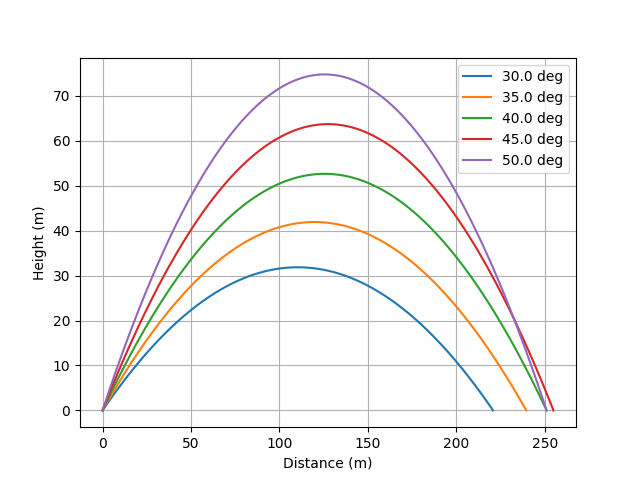
\includegraphics[scale=0.6]{simple}
\end{figure}

\begin{figure}[H]
\centering
\caption{Range as a function of loft angle, no drag or lift}
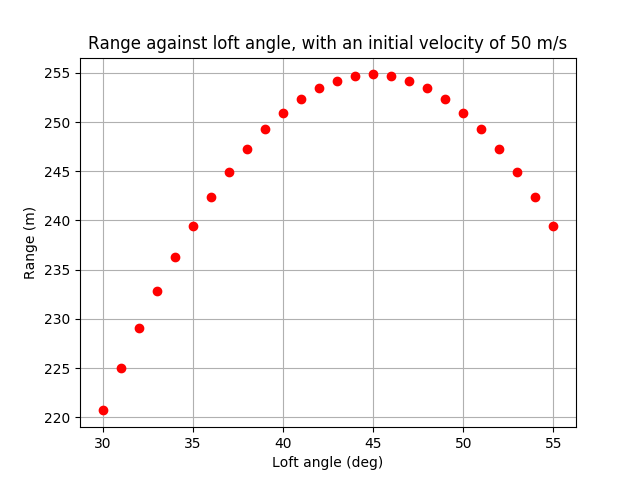
\includegraphics[scale=0.6]{simplerange}
\end{figure}

Figures (1-2) show the maximum range is when the loft angle at 45.0\degree, as predicted by the equations of projectile motion.

\subsubsection{Smooth golf ball experiencing drag}
The drag equation (\ref{drageqn})
\begin{equation} \label{drageqn}
\vec{F_{d}} = \frac{1}{2} A C_{d} \rho_{air} |\vec{v}| \vec{v}
\end{equation}
where $\rho_{air}$ is the density of air; $A$ is the reference area, which in the case of a smooth sphere of radius $r$, is the cross-sectional area $\pi r^2$; $C_d$ is the coefficient of drag, which is dependent on the Reynolds number; and $\vec{v}$ is the flow velocity relative to the golf ball. In this case, we assume the air is stationary and the golf ball is moving through the air with velocity $\vec{v}$.

Applying equation (\ref{drageqn}) to equations (\ref{simpleaccelx}-\ref{simpleaccely}), we get
\begin{equation} \label{dragaccelx}
\frac{\partial v_x}{\partial t}=-k |v_x| v_x
\end{equation}
\begin{equation} \label{dragaccely}
\frac{\partial v_y}{\partial t}=-g-k |v_y| v_y
\end{equation}
where $k=\frac{1}{2} A C_d \rho_{air}$. These equations already do not have a closed-form solution and require numerical methods.
\begin{figure}[H]
\centering
\caption{Golf ball trajectory when experiencing drag but no lift, $C_d$ = 0.5}
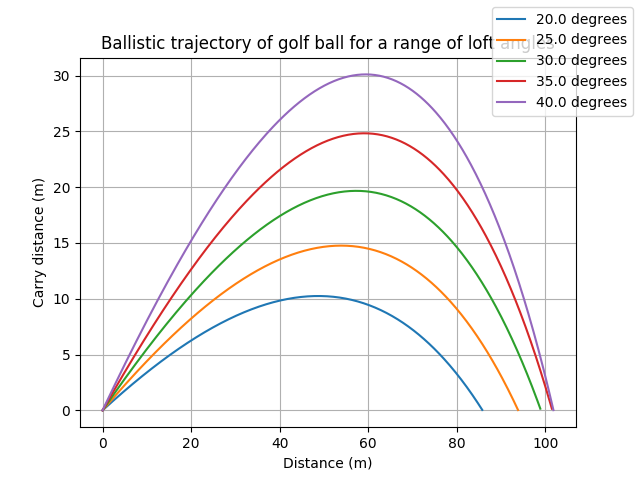
\includegraphics[scale=0.6]{dragcd}
\end{figure}

\begin{figure}[H]
\centering
\caption{Range as a function of loft angle, $C_d$ = 0.5}
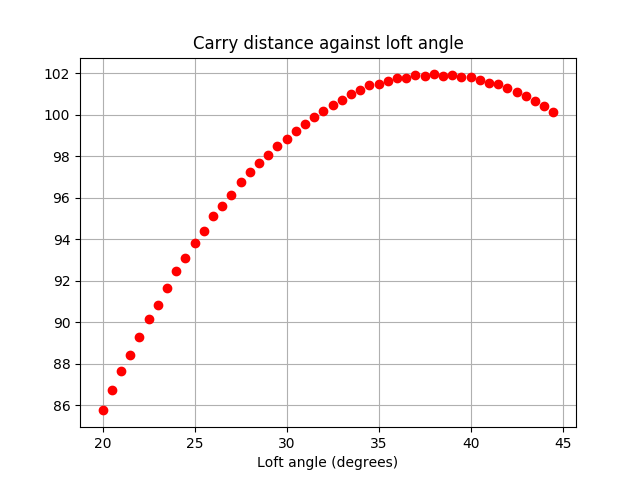
\includegraphics[scale=0.6]{dragcdrange}
\end{figure}

Figure (4) shows that the maximum range is achieved at 40.2\degree, for an initial velocity of \SI{50}{\metre\per\second}. Additionally, the range is significantly decreased when drag was added to the model. The greatest range with drag is about \SI{114}{\metre} versus the previous range of \SI{255}{\metre} at 45.0\degree.
However, $C_d$ is not constant and depends on the Reynolds number, which is proportional to the velocity of the golf ball. The Reynolds number is given by:
\begin{equation} \label{reynolds}
R=\frac{2vr}{\nu}
\end{equation}
where $\nu$ is the kinematic viscosity of air.

Using data from [whereever we found the Reynolds number data], we used Python to construct a quartic fit as shown in Figure (5).\\
A quartic approximation is best as any greater degree would begin to oscillate too much at the edges (Runge's phenomenon). Likewise, a lesser degree would be too linear to give any meaningful relation.\\
One of the limitions of this approach is that we did not have any data above Reynolds number $112,000$ (\SI{38.39}{\meter\per\second}) or below $63,300$ (\SI{21.70}{\meter\per\second}), so the approximation would not hold for those conditions, and may in fact be drastically worse due to the chaotic behaviour of the polynomial at the aforementioned values. To get around this, the coefficient of drag is fixed at 0.8 for Reynolds numbers less than 53,000 and fixed at 0.37 for Reynolds numbers greater than 120,000.

\begin{figure}[H]
\centering
\caption{Coefficient of drag as a function of Reynolds number with curve of best fit}
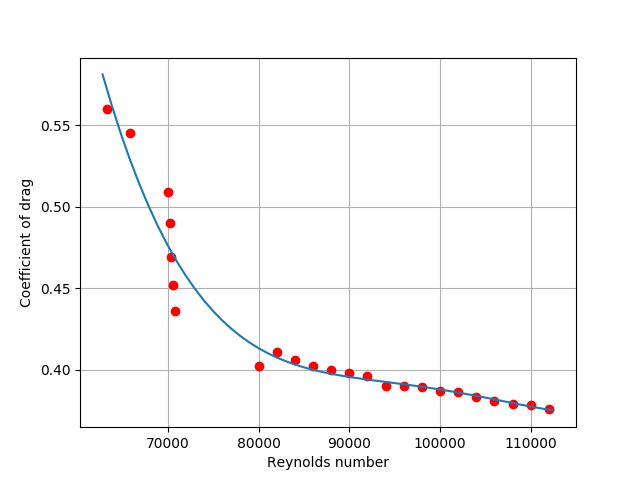
\includegraphics[scale=0.6]{reynolds}
\end{figure}

Applying the approxmation for the coefficient of drag, the optimum loft angle decreases down to about 34.5\degree, shown in figures (6-7).
\begin{figure}[H]
\centering
\caption{Trajectory of golf ball with drag considering Reynolds number, $v_i=$ \SI{50}{\metre\per\second}}
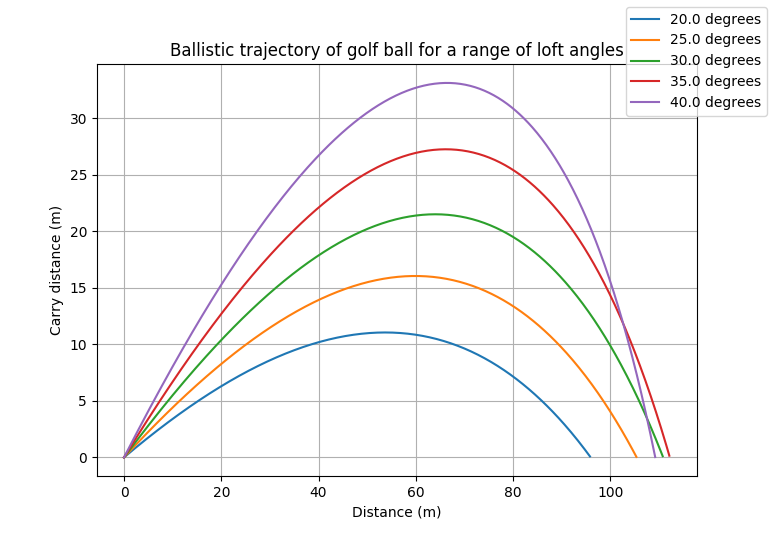
\includegraphics[scale=0.6]{dragwithreynolds}
\end{figure}

\begin{figure}[H]
\centering
\caption{Range against loft angle for golf ball with drag considering Reynolds number, $v_i=$ \SI{50}{\metre\per\second}}
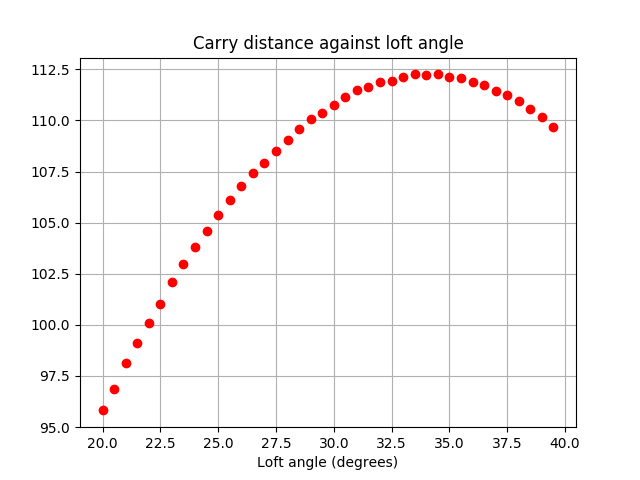
\includegraphics[scale=0.6]{dragwithreynoldsrange}
\end{figure}


\subsubsection{Smooth golf ball experiencing lift}
Lift on a golf ball is caused by the Magnus effect, which is dependent on the backspin of the ball. The equation is similar to the drag equation, however the direction of the force is perpendicular to both angular velocity and translational velocity, unlike in the drag equation.

\begin{equation} \label{lifteqn}
F_l = \frac{1}{2} \rho_{air} C_{l} |v|^2 (\hat{\omega} \times \hat{v})
\end{equation}

where $C_l$ is dependent on the spin parameter of the ball according to [whoever found this equation].
\begin{equation} \label{clifteqn}
C_l = -3.25 S^2 + 1.99 S
\end{equation}
The spin parameter is given by the ratio of the magnitude of tangential velocity to the magnitude of translational velocity.
\begin{equation} \label{spineqn}
S = \frac{r|\omega|}{|v|}
\end{equation}


\bibliography{bibliography}{}
\bibliographystyle{plain}


\end{document}


\grid